\documentclass[12pt]{article}
%\documentclass{nature}

% Including pdf figures
\usepackage{graphicx}
\graphicspath{ {../Plots/} }
\usepackage{pdfpages}
\usepackage{epstopdf}
\epstopdfsetup{outdir=./}
%really place a figure in a location
\usepackage{float}
%Overrun caption
\usepackage[CaptionAfterwards]{fltpage}
% Math stuff
\usepackage{amsmath}
\usepackage{stix}
% Bibliographies
\usepackage[numbers]{natbib}
\bibpunct{(}{)}{,}{a}{}{;} 

\usepackage[flushleft]{threeparttable}

\usepackage[font={scriptsize}]{caption}

\usepackage{lineno} %gives line numbers with \lineno command

\usepackage{setspace}
\onehalfspace

\usepackage{tikz}%for putting words on figures
\usetikzlibrary{positioning}%for relative positioning

%to rotate figures
\usepackage{rotating}
\usepackage{pdflscape}

\begin{document}

\section*{Supplementary Tables}
\renewcommand{\thetable}{S\arabic{table}}

\begin{table}[ht]
\centering
\smallskip
\caption{
Substitutions for different loci orders assuming no interference. %and $r,R\in(0,1/2)$.\textcolor{blue}{write all in form of first line? so that 1/2 cases are okay (can't determine chi if R is 1/2 in second line, or if r is 1/2 in third line}
}
\begin{tabular}{l l}
\hline\hline
  Order of loci &   \\ [0.5ex] \hline
  SDR-A-M & $\rho=r(1-R)+R(1-r)$  \\
  SDR-M-A & $r=\rho(1-R)+R(1-\rho)$ \\ %$\rho=(r-R)/(1-2R)$ \\
  A-SDR-M & $R=r(1-\rho)+\rho(1-r)$ \\ %$\rho=(R-r)/(1-2r)$ \\
  \hline \hline
  \label{tab:chisubstitutions}
 \end{tabular}
\end{table}

\begin{table}[!h]
\centering
\smallskip
\caption{Mean fitnesses and zygotic sex ratio in the resident population ($M$ fixed, XY sex determination). }
\begin{tabular}{l l }
\hline\hline
  Sex \& Life Cycle Stage & Mean Fitness \\ [0.5ex] \hline  \noalign{\vskip 0.5ex}
  female gametes ($\bar{w}_H^\female$) & 
  $p_X^\female w_A^\female + (1-p_X^\female) w_a^\female$ \\ [0.5ex] \hline  \noalign{\vskip 0.5ex}
  X-bearing male gametes ($\bar{w}_{HX}^\male$) & 
  $p_X^{\male} w_A^\male + (1-p_X^{\male}) w_a^\male$ \\ [0.5ex] \hline  \noalign{\vskip 0.5ex}
  Y-bearing male gametes ($\bar{w}_{HY}^\male$) & 
  $p_Y^{\male} w_A^\male + (1-p_Y^{\male}) w_a^\male$ \\ [0.5ex] \hline  \noalign{\vskip 0.5ex}
  male gametes ($\bar{w}_H^\male$) & 
  $(1-q) \bar{w}_{HX}^\male + q \bar{w}_{HY}^\male$ \\ [0.5ex] \hline  \noalign{\vskip 0.5ex}
  females ($\bar{w}^\female$) & 
%  $\begin{array}{l}  (1-\zeta)^{-1} (1-q) \big[ p_X^\female w_A^\female p_X^\male w_A^\male w_{AA}^\female + \\
%  (1 - p_X^\female) w_a^\female p_X^\male w_A^\male w_{Aa}^\female + \\
%  p_X^\female w_A^\female (1 - p_X^\male) w_a^\male w_{Aa}^\female + \\
%  (1-p_X^\female) w_a^\female (1 - p_X^\male) w_a^\male w_{aa}^\female \big] / \left( \bar{w}_H^\female \bar{w}_H^\male \right)
%  \end{array} 
 $\begin{array}{l} \big[ p_X^\female w_A^\female p_X^\male w_A^\male w_{AA}^\female + \\
  (1 - p_X^\female) w_a^\female p_X^\male w_A^\male w_{Aa}^\female + \\
  p_X^\female w_A^\female (1 - p_X^\male) w_a^\male w_{Aa}^\female + \\
  (1-p_X^\female) w_a^\female (1 - p_X^\male) w_a^\male w_{aa}^\female \big] / \left( \bar{w}_H^\female \bar{w}_{HX}^\male \right)
  \end{array}
  $ \\ [0.5ex] \noalign{\vskip 0.5ex} \hline  \noalign{\vskip 0.5ex}
  males ($\bar{w}^\male$) & 
%  $\begin{array}{l} \zeta^{-1} q \big[ p_X^\female w_A^\female  p_Y^\male w_A^\male w_{AA}^\male + \\
%  (1 - p_X^\female) w_a^\female  p_Y^\male w_A^\male w_{Aa}^\male + \\
%  p_X^\female w_A^\female  (1 - p_Y^\male) w_a^\male w_{Aa}^\male + \\
%  (1-p_X^\female) w_a^\female  (1 - p_Y^\male) w_a^\male w_{aa}^\male \big] / \left( \bar{w}_H^\female \bar{w}_H^\male \right) 
%  \end{array}
 $\begin{array}{l} \big[ p_X^\female w_A^\female  p_Y^\male w_A^\male w_{AA}^\male + \\
  (1 - p_X^\female) w_a^\female  p_Y^\male w_A^\male w_{Aa}^\male + \\
  p_X^\female w_A^\female  (1 - p_Y^\male) w_a^\male w_{Aa}^\male + \\
  (1-p_X^\female) w_a^\female  (1 - p_Y^\male) w_a^\male w_{aa}^\male \big] / \left( \bar{w}_H^\female \bar{w}_{HY}^\male \right) 
  \end{array}
  $ \\ [0.5ex] \noalign{\vskip 0.5ex} \hline  \noalign{\vskip 0.5ex}
  fraction zygotes male ($\zeta$) & $q \left[ p_Y^\male w_A^\male+(1-p_Y^\male)w_a^\male\right] / \bar{w}_H^\male $
   \\ [0.5ex]  \noalign{\vskip 0.5ex}
  \hline \hline
  \label{tab:meanfitnesses}
 \end{tabular}
\end{table}

\newpage
\section*{Supplementary Figures}
\renewcommand{\thefigure}{S\arabic{figure}}

%%%%%%%%%%%%%%%%%%%%%%%%%%%%%%%%%%%%%%%%%%%%%%%%%%%%%%%%%
%Both neo-W haplotypes can spread, in the absence of haploid selection, when there is overdominance
%%%%%%%%%%%%%%%%%%%%%%%%%%%%%%%%%%%%%%%%%%%%%%%%%%%%%%%%%
\begin{figure}[!h]
\centering
\centerline{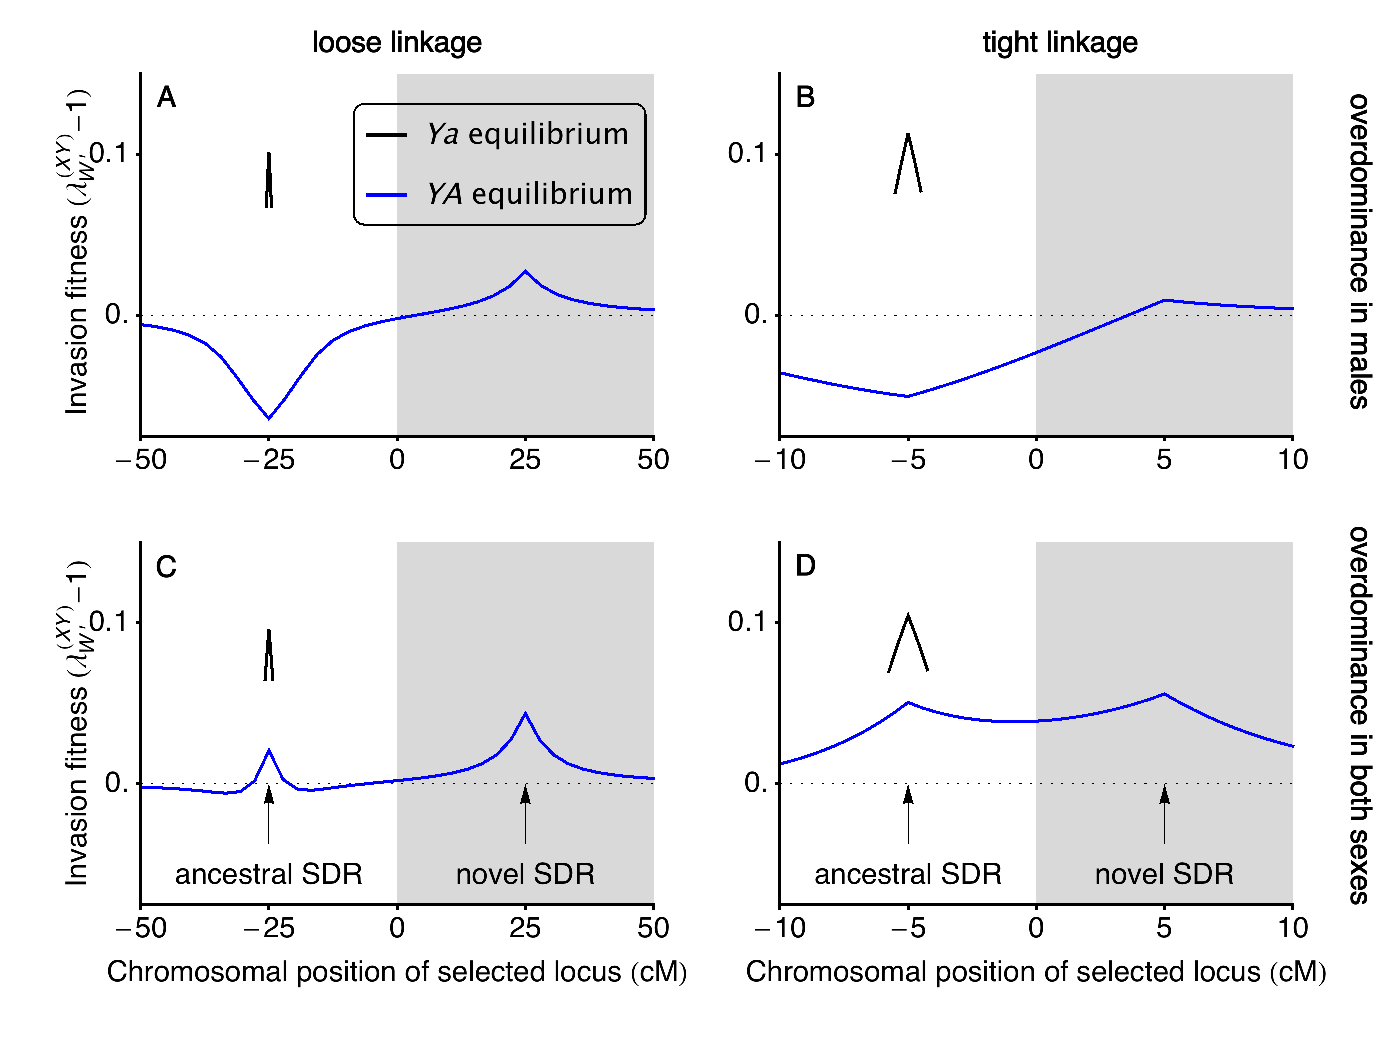
\includegraphics[width=\linewidth]{PositionPlot_Overdominance.eps}}
\caption{
%Neo-W alleles can spread when loci under diploid selection are tightly linked to the ancestral sex determining locus ($r\approx0$). 
%In panels A and B, the $a$ allele is favoured in females ($w_{aa}^\female=1.05$, $w_{Aa}^\Hermaphrodite=1$, $w_{AA}^\female=0.85$) and selection in males is overdominant ($w_{aa}^\male=w_{AA}^\male=0.75$).
%In panels C and D, selection in males and females is overdominant ($w_{aa}^\female=w_{AA}^\female=0.6$, $w_{aa}^\male=0.5$, $w_{AA}^\male=0.7$, $w_{Aa}^\Hermaphrodite=1$).
%There is no haploid selection $t^\Hermaphrodite = \alpha^\Hermaphrodite_\Delta = 0$.
%These parameters are marked by daggers in Figure \ref{fig:regionplots}B and C, which show that neo-W invasion is expected for any $R$ ($\lambda_{W'A}^{(XY)},\lambda_{W'a}^{(XY)}>1$) when the $a$ allele is nearly fixed on the Y (black lines in this figure; not stable for $r>>0$). 
%Equilibria where the $A$ allele is more common among Y-bearing male gametes can also be stable and allow neo-W invasion for these parameters (blue lines). 
%The weak selection approximation holds when all recombination rates are large relative to selection (around 0 in panels A and C), in which case, in the absence of haploid selection, neo-W alleles should spread if and only if they are more tightly linked to the selected locus (positive invasion fitness if and only if the selected locus is in the grey region). 
%However, when linkage is tight (panels B and D and when the selected locus is near the SDRs in all panels), this weak selection prediction can break down. 
}
\label{fig:positionOverdominance}
\end{figure}

\newpage

%%%%%%%%%%%%%%%%%%%%%%%%%%%%%%%%%%%%%%%%%%%%%%%%%%%%%%%%%
%Both neo-W haplotypes can spread, in the absence of haploid selection, when there is overdominance
%%%%%%%%%%%%%%%%%%%%%%%%%%%%%%%%%%%%%%%%%%%%%%%%%%%%%%%%%
\begin{figure}[!h]
\centering
\centerline{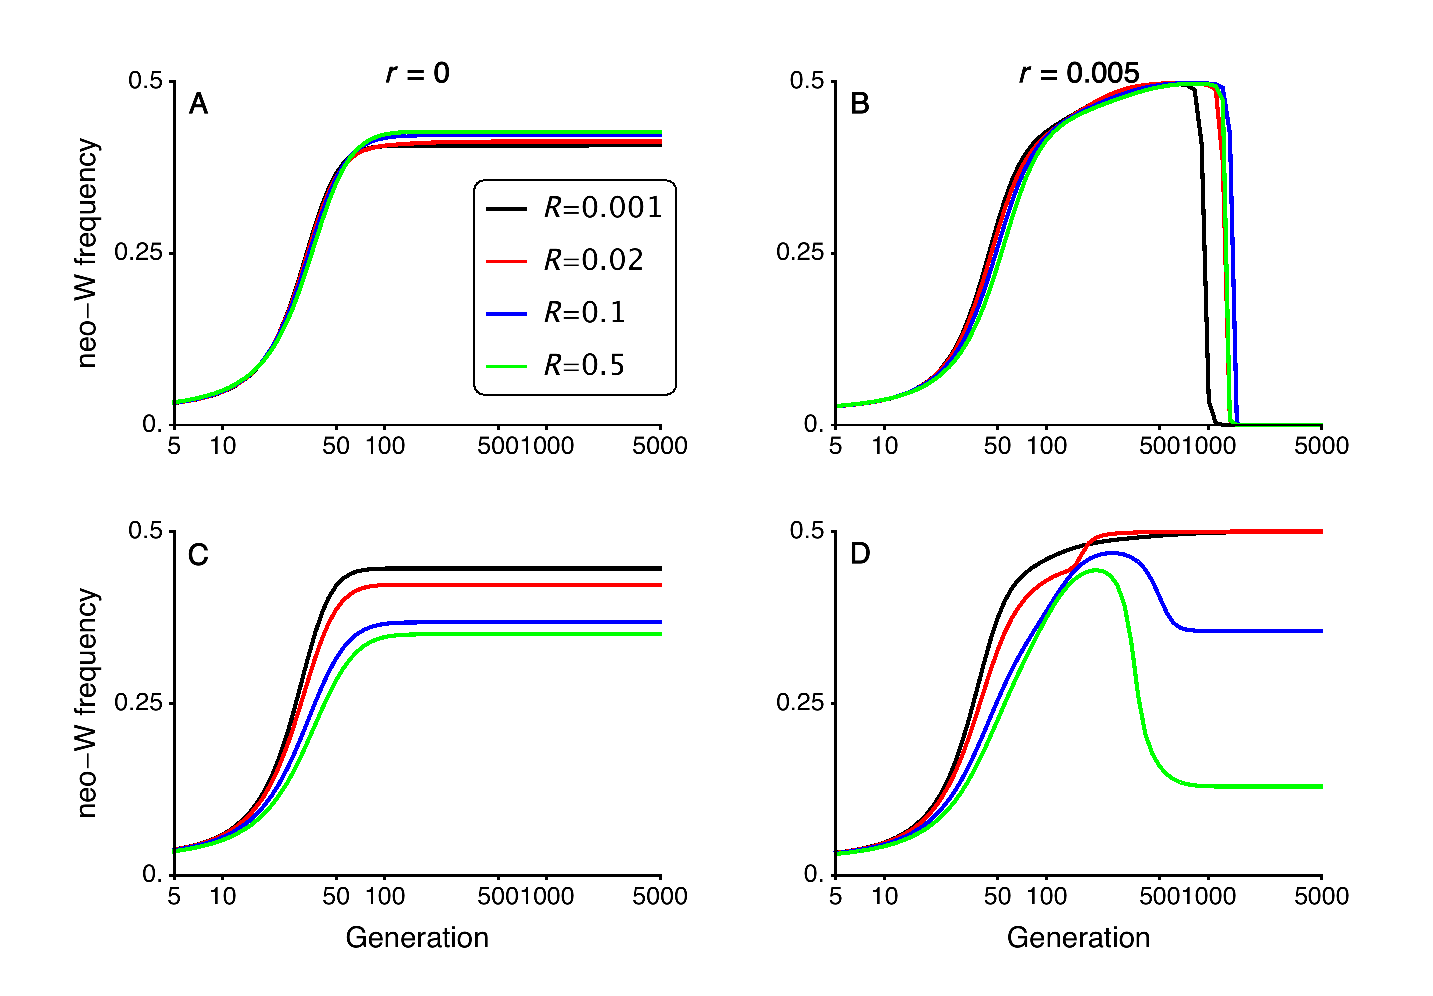
\includegraphics[width=\linewidth]{Temporal_Overdominance.eps}}
\caption{
%Following invasion by a neo-W allele, there can be a complete transition to a new sex-determination system, maintenance of polymorphism at both ancestral-XY and neo-ZW sex determining regions, or loss of the new sex-determining allele. 
%Here we plot the frequency of the neo-W allele among female gametes; as the neo-W reaches frequency $0.5$, polymorphism at the ancestral XY locus is lost with Y becoming fixed such that sex is determined only be the ZW allele carried by a female gamete. 
%Panels A, C and D show cases where a steady state is reached with the neo-W at a frequency below $0.5$, in which case ancestral-X and Y alleles also both segregate. 
%In all cases, we assume that the $a$ allele is initially more common than the $A$ allele on the Y (Y-$a$ is fixed when $r=0$). 
%When $r>0$ (panels B and D), Y-$A$ haplotypes created by recombination can become more common than Y-$a$ haplotypes as the neo-W spreads.
%In B, this leads to loss of the neo-W and the system goes to an equilibrium with X-$a$ and Y-$A$ haplotypes fixed (equilibrium $A'$), such that all females have the high fitness genotype $aa$ and all males are $Aa$. 
%For the parameters in B, neo-W alleles have negative invasion fitness when the Y-$A$ haplotype is ancestrally more common than Y-$a$ (see blue lines in Figure \ref{fig:positionOverdominance}A and  \ref{fig:positionOverdominance}B near the ancestral SDR). 
%In contrast, the neo-W is not lost in panel D as it is favoured near $r\approx0$ (see blue lines in Figure \ref{fig:positionOverdominance}C and  \ref{fig:positionOverdominance}D near the ancestral SDR). 
%Fitness parameters are the same as in Figure \ref{fig:positionOverdominance}; in panels A and B the $a$ allele is favoured in females ($w_{aa}^\female=1.05$, $w_{Aa}^\Hermaphrodite=1$, $w_{AA}^\female=0.85$) while there is overdominance in males ($w_{aa}^\male=w_{AA}^\male=0.75$) and in panels C and D, there is overdominance in both sexes ($w_{aa}^\female=w_{AA}^\female=0.6$, $w_{aa}^\male=0.5$, $w_{AA}^\male=0.7$, $w_{Aa}^\Hermaphrodite=1$). 
%These parameters are marked by a dagger in Figure \ref{fig:regionplots}. 
%Here, there is no haploid selection $t^\Hermaphrodite = \alpha^\Hermaphrodite_\Delta = 0$.
}
\label{fig:temporalOverdominance}
\end{figure}

\begin{figure}[!h]
\centering
\centerline{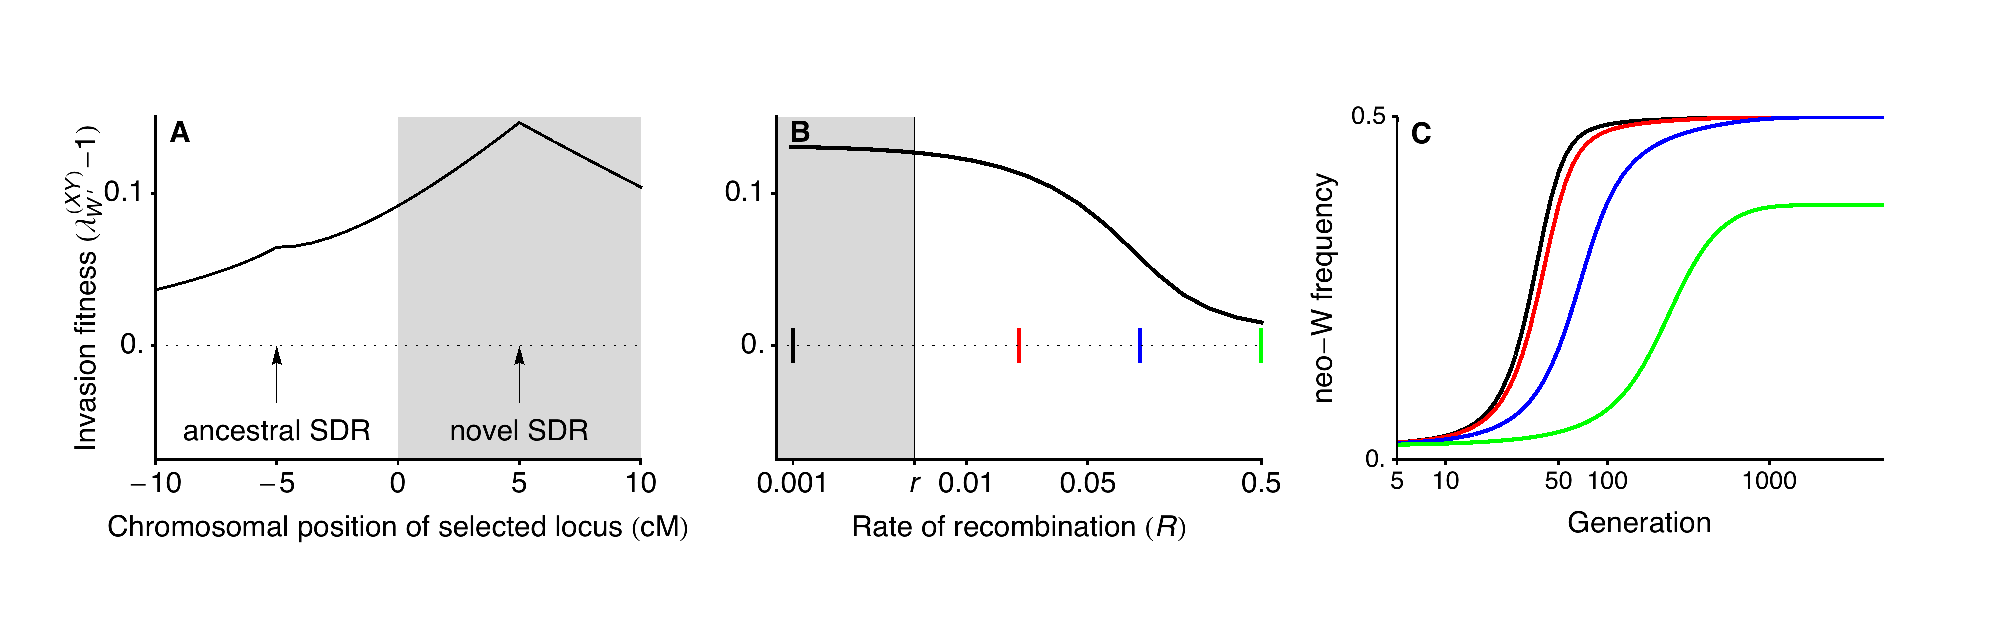
\includegraphics[width=1.5\linewidth]{PositionPlot_SexAntagTighter_MaleDrive.eps}}
\caption{
%When there is sexually-antagonistic selection and haploid selection, a neo-W may invade for any $R$.
%Panel A shows that the invasion fitness of a neo-W is positive where linkage is tight, even when $r<R$ (unshaded region).
%In panel B, we vary the recombination rate between the neo-W and the selected locus ($R$) for a fixed recombination rate between the ancestral-SDR and the selected locus ($r=0.005$).
%Coloured markers show recombination rates for which the temporal dynamics of neo-W invasion are plotted in panel C (black $R=0.001$, red $R=0.02$, blue $R=0.1$, green $R=0.5$). 
%The diploid selection parameters used in this plot are the same as in Figure \ref{fig:SexAntagTighter}. 
%There is also meiotic drive in males favouring $a$ ($\alpha_{\Delta}^\male=-0.08$), this full set of parameters is marked by an asterisk in Figure \ref{fig:regionMaleDrive}A.
%When $R=0.5$ (green curve), the neo-W does not reach fixation and X,Y,Z, and W alleles are all maintained in the population, see Figure \ref{fig:freqAll}C.
}
\label{fig:SexAntagTighterMaleDrive}
\end{figure}

\begin{figure}[!h]
\centering
\centerline{\includegraphics[width=\linewidth]{Region_Plot_combined_MaleDrive.eps}}
\caption{
%Meiotic drive in males affects whether neo-W-$A$ and neo-W-$a$ haplotypes spread when the ancestral-XY locus is tightly linked to a locus under selection ($r=0$). 
%We vary the fitness of male homozygotes relative to heterozygotes ($w_{Aa}^\Hermaphrodite=1$) and only consider stable equilibria at which both \textbf{A} locus allele are maintained and the $a$ allele is initially fixed on the Y, region outlined. 
%In panels A-C, meiotic drive in males favours the $a$ allele ($\alpha_{\Delta}^\male=-0.16$), creating male-biased sex ratios and generally increasing $\lambda_{WA}$ and $\lambda_{Wa}$. 
%By contrast, $\lambda_{W'A}^{(XY)}$ and $\lambda_{W'a}^{(XY)}$ tend to be reduced when meiotic drive in males favours the $A$ allele ($\alpha_{\Delta}^\male=0.16$), panels D-F. 
%We consider three forms of selection in females: directional selection in favour of the $A$ allele (panels A and D, $w_{aa}^\female=0.85$, $w_{AA}^\female=1.05$), direction selection in favour of the $a$ allele (panels B and E, $w_{aa}^\female=1.05$, $w_{AA}^\female=0.85$), and overdominance (panels C and F, $w_{aa}^\female=w_{AA}^\female=0.6$).
%\textcolor{red}{Panel F mislabelled, should have $\lambda_{Wa}>1$ \& $\lambda_{WA}<1$ as the upper label that has the line.}
}
\label{fig:regionMaleDrive}
\end{figure}

\newpage
\begin{figure}[!h]
\centering
\centerline{\includegraphics[width=\linewidth]{Region_Plot_combined_MaleGS.eps}}
\caption{
%Parameters for which neo-W-$A$ and neo-W-$a$ haplotypes spread when there is male gametic competition at a locus that is tightly linked to the ancestral-XY locus.
%Diploid selection parameters ($w_{ij}^\Hermaphrodite$) are the same as those in Figure \ref{fig:regionMaleDrive}. 
%The $a$ allele is favoured during male gametic competition in Panels A-C ($w_{a}^\male=1.16$, $w_{A}^\male=1$), which creates male biased sex ratios and increases $\lambda_{W'A}^{(XY)}$ and $\lambda_{W'a}^{(XY)}$. 
%On the other hand, the $A$ allele is favoured during male gametic competition in Panels D-F ($w_{a}^\male=1$, $w_{A}^\male=1.16$) and $\lambda_{W'A}^{(XY)}$ and $\lambda_{W'a}^{(XY)}$ tend to be reduced. 
%Compared to the meiotic drive parameters in Figure \ref{fig:regionMaleDrive}, the effect of these male gametic competition parameters on the sex ratio is smaller. 
%For example, in Figure \ref{fig:regionMaleDrive}A-C, the ancestral sex ratio is $\alpha^\male=0.58$ at equilibrium (B) and in panels A-C of this plot, the ancestral sex ratio is $w_{a}^\male/(w_{A}^\male+w_{a}^\male)=0.537$ at equilibrium (B). 
}
\label{fig:regionMaleGS}
\end{figure}

\begin{figure}[!h]
\centering
\centerline{\includegraphics[width=\linewidth]{Region_Plot_combined_FemaleDrive.eps}}
\caption{
%Parameters for which neo-W-$A$ and neo-W-$a$ haplotypes spread when there is female meiotic drive at a locus that is tightly linked to the ancestral-XY locus.
%Diploid selection parameters ($w_{ij}^\Hermaphrodite$) are the same as those in Figure \ref{fig:regionMaleDrive} and \ref{fig:regionMaleGS}. 
%The $a$ allele is favoured by meiotic drive in females in Panels A-C ($\alpha_{\Delta}^\female=-0.16$), which increases $\lambda_{W'a}^{(XY)}$ and decreases $\lambda_{W'A}^{(XY)}$. 
%Female meiotic drive in favour of the $A$ allele (panels D-F, $\alpha_{\Delta}^\female=-0.16$) has the opposite effect. 
}
\label{fig:regionFemaleDrive}
\end{figure}

\begin{figure}[!h]
\centering
\centerline{\includegraphics[width=\linewidth]{Region_Plot_combined_FemaleGS.eps}}
\caption{
%Parameters for which neo-W-$A$ and neo-W-$a$ haplotypes spread when there is female gametic competition at a locus that is tightly linked to the ancestral-XY locus.
%Diploid selection parameters ($w_{ij}^\Hermaphrodite$) are the same as those in Figure \ref{fig:regionMaleDrive}, \ref{fig:regionMaleGS}, and \ref{fig:regionFemaleDrive}. 
%The $a$ allele is favoured during female gametic competition in females in Panels A-C ($w_{a}^\female=1.16$, $w_{A}^\female=1$), which increases $\lambda_{W'a}^{(XY)}$ and decreases $\lambda_{W'A}^{(XY)}$. 
%The $A$ allele is favoured during gametic competition in panels D-F ($w_{a}^\female=1$, $w_{A}^\female=1.16$), giving the opposite effect on $\lambda_{W'a}^{(XY)}$ and $\lambda_{W'A}^{(XY)}$. 
}
\label{fig:regionFemaleGS}
\end{figure}

\begin{landscape}
\begin{figure}[!h]
\centering
\centerline{
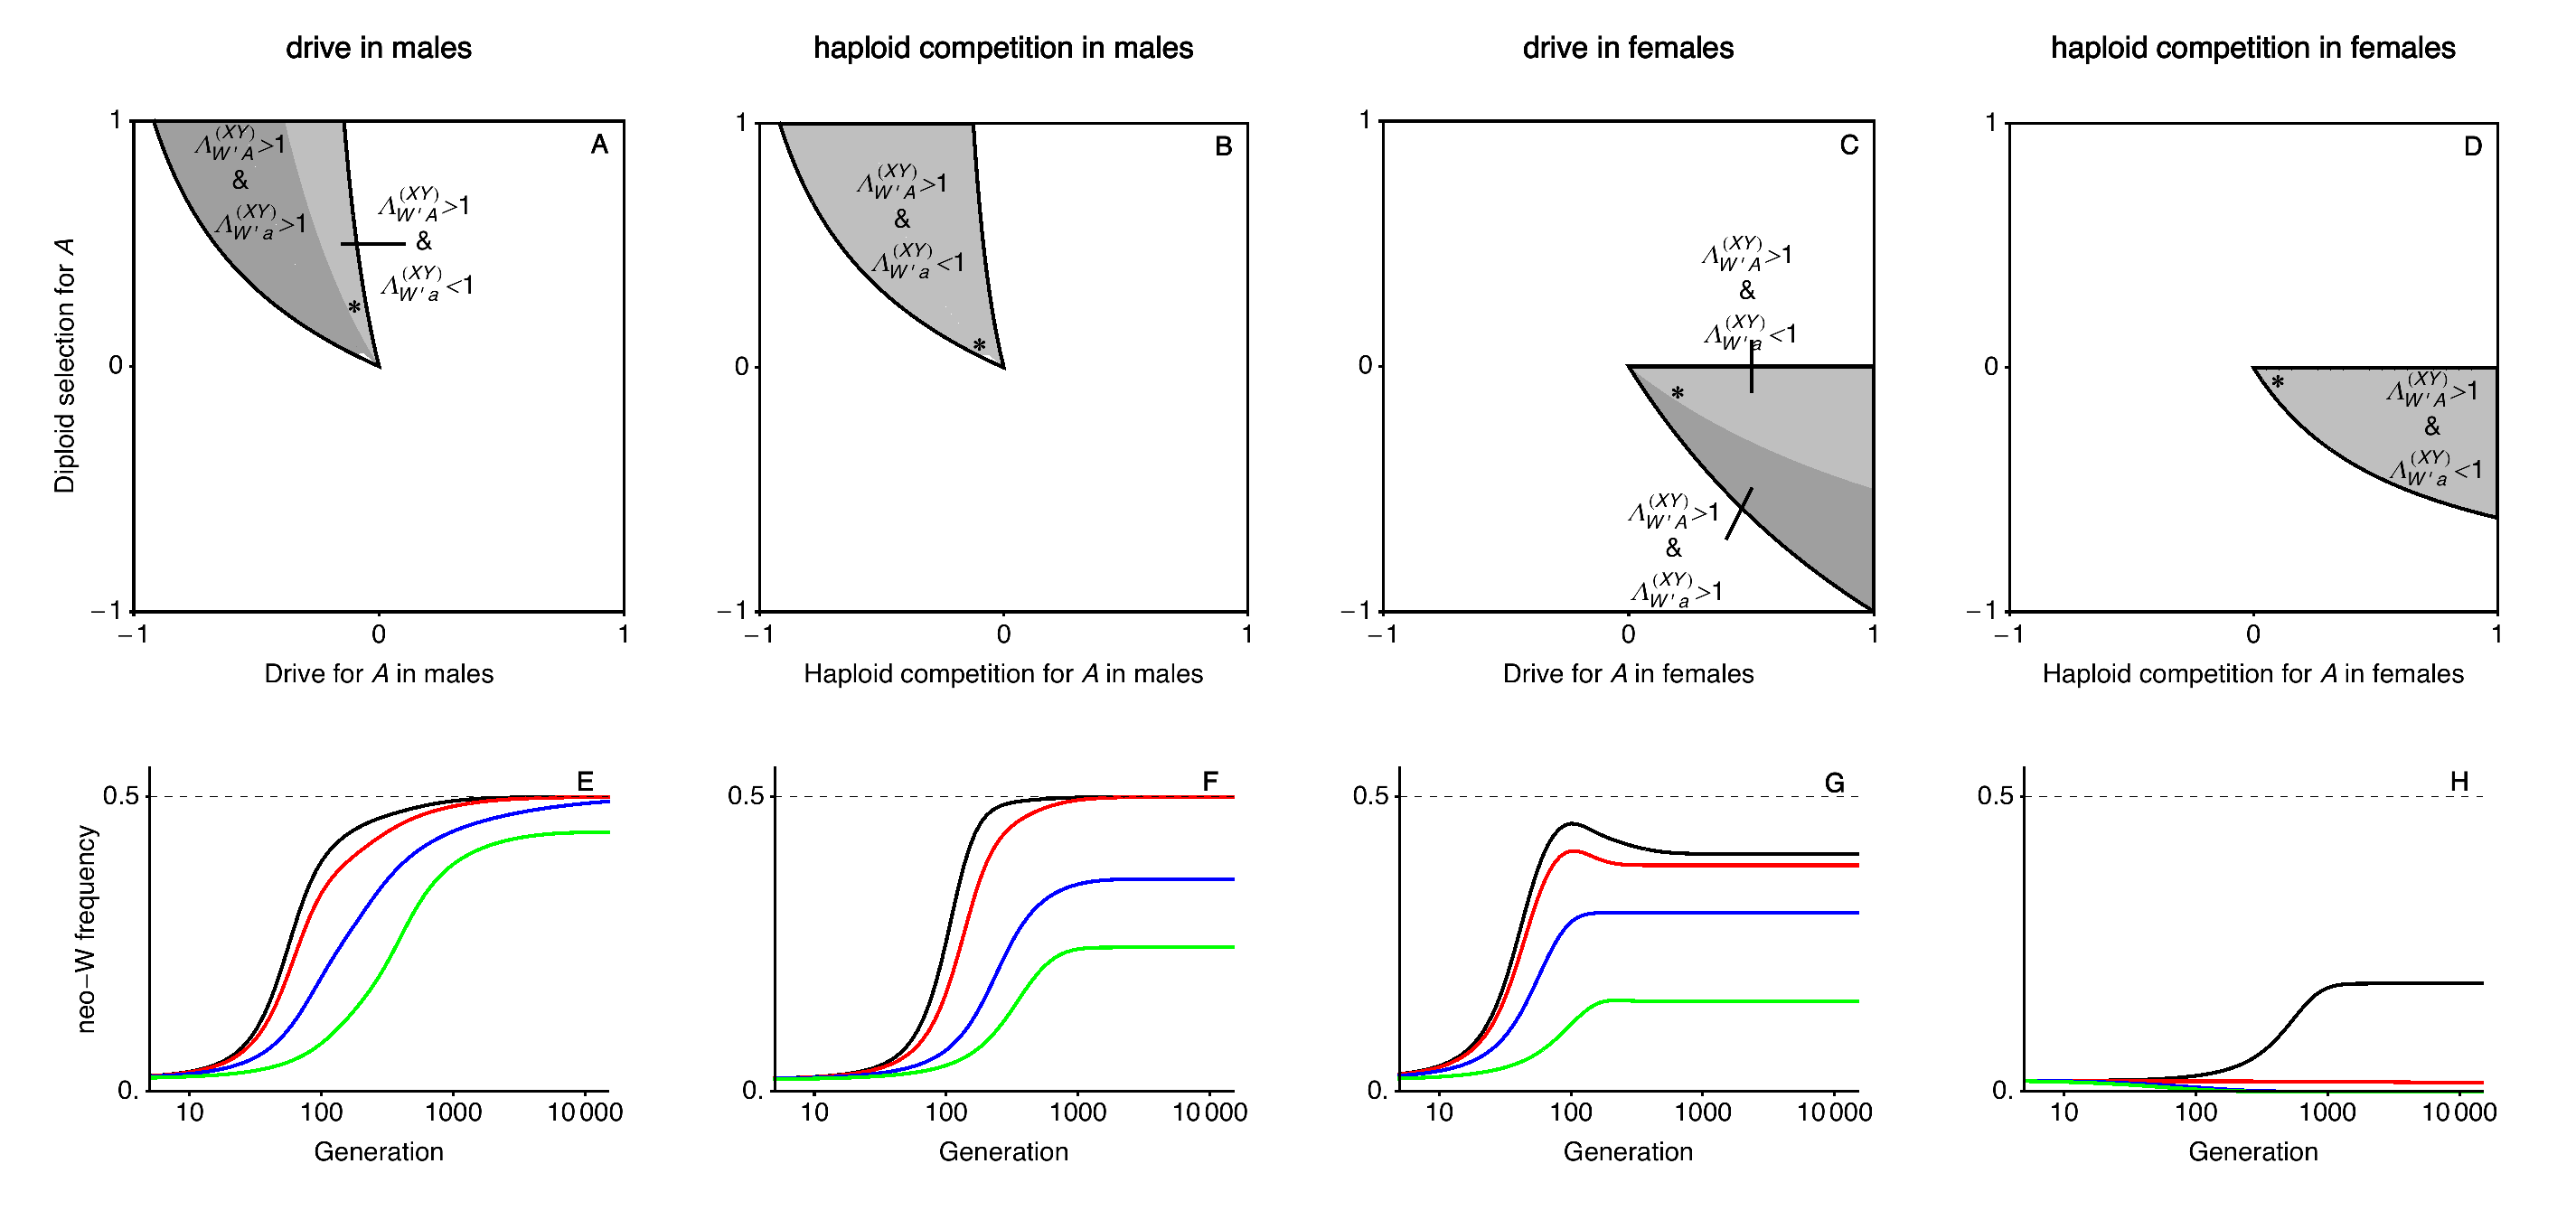
\includegraphics[width=\linewidth]{All_plot_combined_PloidAntag.eps}
}
\caption{
%A-D show when each of the neo-W haplotypes invade an internally stable equilibrium with $a$ fixed on the Y (found by setting $r=0$).
%The y-axis shows directional selection in diploids of both sexes, $s^\female=s^\male$, and the x-axes show sex-specific drive, $\alpha_\Delta^\Hermaphrodite$, or haploid competition, $t^\Hermaphrodite$.
%The top left and bottom right quadrants therefore imply ploidally-antagonistic selection (and these are the only places where neo-W haplotypes can invade).
%Dominance is equal in both sexes, $h^\female=h^\male=3/4$. 
%E-F show the temporal dynamics of neo-W frequency in females with parameters given by the asterisks in the corresponding A-D plot, with $r=1/200$, for four different $R$.
%Black $R=1/1000$, Red $R=2/100$, Blue $R=1/10$, Green $R=1/2$.  
%Dashed line in E-H gives ``fixation" of neo-W (all females heterozygous ZW).
}
\label{fig:regionPloidAntag}
\end{figure}
\end{landscape}

%\begin{landscape}
\begin{figure}[!h]
\centering
\centerline{
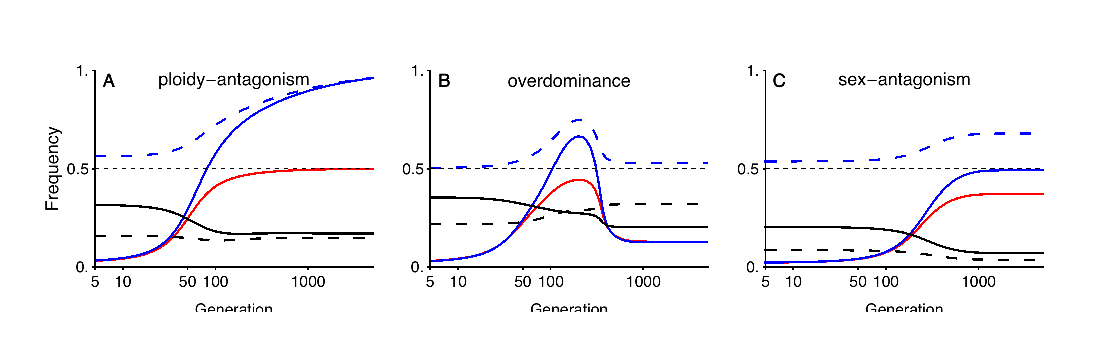
\includegraphics[width=\linewidth]{Freq_plot_combined_PloidAntag.eps}
}
\caption{
%Fixation of neo-W or maintenance of multiple sex-determining systems. 
%The curves show the frequencies of the neo-W (red), ancestral-Y (blue), and $A$ allele (black) among female gametes (solid curves) and among male gametes (dashed curves). 
%In panel A, there is a complete transition from XY sex determination (XX-ZZ females and XY-ZZ males) to ZW sex determination (YY-ZW females and YY-ZZ males).  
%In panels B and C a polymorphism is maintained at both the ancestral XY locus and the neo-ZW locus, such that there are males with genotypes XY-ZZ or YY-ZZ and females with genotypes XX-ZZ, XX-ZW, XY-ZW, or YY-ZW. 
%In panel A, selection is ploidally antagonistic with drive in males (parameters as in the green curve in Figure \ref{fig:SexRatioBad}B).
%In panel B, there is overdominance in both sexes and no haploid selection (parameters as in the green curve in Figure \ref{fig:temporalOverdominance}C).
%In panel C, there is sexually-antagonistic selection in diploids with drive in males (parameters as in the green curve in Figure \ref{fig:regionMaleDrive}C).
%%In Panel D there is ploidally-antagonistic selection with haploid competition in males (parameters as in the green curve of Figure \ref{fig:regionPloidAntag}F).
%In all cases, the initial equilibrium frequency has $a$ near fixation on the Y.
}
\label{fig:freqAll}
\end{figure}
%\end{landscape}

\end{document}



